\documentclass{article}
\usepackage{amsmath, graphicx}
\title{A Parameter-Tuned Monte Carlo Prediction Model for the 2012 U.S. Presidential Election}
\date{November 4th, 2012}
\author{Jared Park \& Swupnil Sahai\\ Department of Statistics\\ University of California, Berkeley}
\begin{document}
\parindent 31pt
\maketitle

%ABSTRACT
\begin{abstract}
We model the upcoming U.S. presidential election utilizing a Bayesian framework in combination with Markov Chain Monte Carlo methods as provided by rJAGS. Our primary data set consists of polling data from throughout the entire year prior to the elections in 2004, 2008, and 2012, in addition to the actual popular vote results in 2004 and 2008. After attempting to predict the 2004 and 2008 elections, we find that prediction accuracy is maximized when we only consider (for each state) the 30 polls taken most closely in time to election day, rather than all of the available polling data. Utilizing an informative prior that takes into account the results of the 2004 and 2008 elections, our analysis indicates that President Obama has a 99.9\% chance of winning the 2012 presidential election, and that he is expected to win with 303 electoral votes.
\end{abstract}

%INTRO
\pagebreak
\section{Introduction}

\hspace{31pt} Election prediction in the United States is attempted by scientists across the country and the world, with statisticians utilizing methodologies across the entire Frequentist-Bayesian spectrum. The U.S. presidential election in particular raises interesting challenges as the voting dynamic in every state is different, requiring the construction of complex models that take into account the nuances in voting behavior. Each state's historical voting trends, however, also provide information that can greatly increase  accuracy if incorporated into a prediction model (Rigdon, 2009). As a frequentist approach cannot necessarily incorporate this prior information, we elect to utilize a Bayesian methodology to predict the 2012 U.S. presidential election.\\
\indent Our framework uses a Bayesian estimator that allows one to apply both prior and current information for each state to determine each candidate's probability of winning that state in the presidential election. The estimators incorporate both the previous election�s results (to capture each state's party tendency) and current polling data (to capture each state's current candidate tendency).\\
\indent As such, we utilize an informative prior based on long-term voting trends within a state and different probability distributions, as has been explored before. Once we estimate the probability that a candidate will win a state, these values can be used to determine the probability that each candidate will win the election by using a Monte Carlo simulation. The idea of using Bayesian estimation rather than frequentist estimation techniques has been explored by others (Jackman \& Rivers, 2001; Kaplan \& Barnett, 2003), but we use the 2008 data to take an active approach to tuning the parameters of the MC chains, as well as tuning the number of polls that are actually considered in the likelihood function.\\
\indent Our article is organized as follows. The next section provides a discussion of the polling data set used for our prediction. Next, we describe the Bayesian methodology used to estimate each candidate's probability of winning each state's Electoral College votes. The following section uses these estimators, coupled with our polling data, to retrospectively provide a prediction and analysis of the 2008 U.S. presidential election. Lastly, we discuss the results regarding the 2012 election.

%DATA
\pagebreak
\section{Data}
\hspace{31 pt} For each of 2004, 2008, and 2012, we utilized publicly available polling data (from various polling agencies in each state) throughout the year prior to the election. We opted not to utilize economic data such as unemployment as we believe the effects of these factors are already captured by polling data. As such, the comprehensive polling data matrix for a given election consists of four columns: (A) the date the poll was taken, (B) the percentage of responses in favor of the Democratic candidate, (C) the percentage of responses in favor of the Republican candidate, and (D) the total number of responses for the particular poll. 

%METHODOLOGY
\section{Methodology}

%LIKELIHOOD
\subsection{Likelihood}
\hspace{31pt} Let $p_{ij}$ denote the true proportion of voters in state $j$ who are voting for candidate $i$ in the election (for simplicity, let i = 1 correspond to the Democratic candidate, i=2 correspond to the Republican candidate, i = 3 collectively correspond to all third-party candidates or to voters who have declared that they are still undecided). To obtain an expression for the likelihood function, we then let $\bf{X_j}$ = $(X_{1j},X_{2j}, X_{3j})$ denote the random vector of sample proportions obtained from a poll in state $j$. Then, if the poll for state $j$ has $n_j$ respondents, it follows that $\bf{X_j}$ = $(X_{1j},X_{2j}, X_{3j}) \sim$ Multinomial $(n_j, p_{1j},p_{2j},p_{3j})$, and the joint probability density of $\bf{X_j}$ is:
\begin{equation}
g_j({\bf X_j|p_j}) = \frac{n_j!}{x_{1j}!x_{2j}!x_{3j}!}p_{1j}^{x_{1j}}p_{2j}^{x_{2j}}p_{3j}^{x_{3j}}
\end{equation}
\indent Finally, if we let $k_j$ denote the number of polls available for state j, we create a comprehensive polling matrix ${\bf A_j = (X_j^1,\dots,X_j^{k_j})^T}$. In the past, other authors have generally treated ${\bf A_j}$ = all available polling data for state $j$ in an effort to utilize as much information as possible; we, however, found that it would be more optimal to limit the range of our polling data with a modified ${\bf A_j' \subset A_j}$. The details of how we chose this optimal subset of data from the comprehensive polling data is discussed in {\bf3.6 Parameter Tuning}.

%PRIOR
\subsection{Informative Prior}
\hspace{31pt} Now the joint prior distribution of the true voting proportions in state j is $\bf{p_j}$ = $(p_{1j},p_{2j},p_{3j}) \sim$ Dirichlet($b_{1j},b_{2j},b_{3j}$), where a Dirichlet distribution is chosen to allow for conjugacy. Hence, the joint probability density function for state $j$ can be written as:
\begin{equation} \label{eq:prior}
f_j(p_{1j},p_{2j},p_{3j}) = c_jp_{1j}^{b_{1j}-1}p_{2j}^{b_{2j}-1}p_{3j}^{b_{3j}-1}
\end{equation}
\begin{equation}
p_{ij} \geq 0 \textrm{ for }  i=1,2,3; \sum\limits_{i=1}^3 p_{ij} = 1
\end{equation}
\noindent where $c_j = \Gamma(\sum_{i=1}^3 b_{ij})/\prod_{i=1}^3\Gamma(b_{ij})$.

\indent Now to find the marginals of this distribution, we first rewrite the density function so that there are only two parameters and then we integrate over $p_{2j}$, as follows:
\begin{equation}
f_{1j}(p_{1j}) = \int_0^{1-p_{1j}} c_jp_{1j}^{b_{1j}-1}p_{2j}^{b_{2j}-1}(1-p_{1j}-p_{2j})^{b_{3j}-1} dp_{2j} 
\end{equation} 
\begin{equation}
= c_jp_{1j}^{b_{1j}-1} \int_0^{1-p_{1j}} p_{2j}^{b_{2j}-1}(1-p_{1j}-p_{2j})^{b_{3j}-1} dp_{2j} 
\end{equation} 
\begin{equation}
= c_{j}' p_{1j}^{b_{1j}-1}(1-p_{1j})^{b_{2j}+b_{3j}-1}, 0 \leq p_1\leq 1 
\end{equation}\\
where $c_{j}' = c_j \frac{\Gamma(b_{2j})\Gamma(b_{3j})}{\Gamma(b_{2j}+b_{3j})} =  \frac{\Gamma(\sum_{i=1}^3 b_{ij})}{\Gamma(b_{1j})\Gamma(b_{2j}+b_{3j})}$.
Due to the symmetry of the Dirichlet joint distribution, it follows that for each $i$ and each $j$:
\begin{equation} \label{eq:beta}
f_{ij}(p_{ij}) \sim \textrm{ Beta}(b_{ij}, \sum\limits_{k=1}^3b_{kj} - b_{ij}).
\end{equation}

\indent Hence, to create an informative Beta prior over each $p_{ij}$, we assigned a hyperparameter $b_{ij}$ equal to a weighted average of $\hat p_{ij}^{2008}$ and $\hat p_{ij}^{2004}$, the true proportions of voters in state $j$ who voted for category $i$ in 2004 and in 2008. Furthermore, each hyperparatmer was multiplied by a constant of 50 to ensure $\sum_{k=1}^3p_{kj} = 50$ in an effort to create optimal variance in each of the marginal Beta distributions as formulated in (7). As such, we calculated, in the framework of equation (2), that:
\begin{equation}
b_{ij} = (0.5\cdot\hat p_{ij}^{2004} + 0.5\cdot\hat p_{ij}^{2008})\cdot 50, \textrm{ for } i \leq 2
\end{equation}
\begin{equation}
b_{ij} = 50-b_{1j}-b_{2j}, \textrm{ for } i =3
\end{equation}

%DATA ADJUSTMENTS
\subsection{*Informative Prior Data Adjustments}
\hspace{31pt} When using an informative formulation of the hyperparameters, we found that there were some states that had a 0\% prior probability of undecided or third-party voters (i.e. $b_{3j}=0$), in which case the prior probability $b_{3j}$ was adjusted to 0.01. Additionally, to ensure that $\sum_{i=1}^3b_{ij} = 50$, the hyperparameters for the votes going to the Democratic candidate ($b_{1j}$) and the Republican candidate ($b_{2j}$) were  decreased by 50$\cdot$0.005 in this case. Hence, for the special case when $b_{3j}=0$, we used the following adjusted hyperparameters:
\begin{equation}
b_{ij}' = (0.5\cdot\hat p_{ij}^{2004} + 0.5\cdot\hat p_{ij}^{2008} - 0.005)\cdot 50, \textrm{ for } i \leq 2
\end{equation}
\begin{equation}
b_{ij}' = 0.01\cdot 50, \textrm{ for } i =3
\end{equation}

%HIERARCHICAL MODEL
\subsection{*Prior with Hierarchical Model}
\hspace{31pt} To account for the possible interstate dependence of voting tendencies, a hierarchical model could also be utilized such that the prior Dirichlet distributions for each state are identical. This is formulated by creating identical hyperparamaters on the hyper prior distribution of  $b_{ij}$. In this case, we have:
\begin{equation}
b_{ij} \sim \textrm{ Gamma}(0.5\cdot\hat p_{i\cdot}^{2004} + 0.5\cdot\hat p_{i\cdot}^{2008}, \frac{1}{4} (\textrm{Var } p_{i\cdot}^{2004} + \textrm{Var } p_{i\cdot}^{2008})).
\end{equation}
where $\textrm{Var } p_{i\cdot}^{200k}$ is a measure of the variance of polling samples in the year 200$k$.
\indent In general, however, we found that such a hierarchical model provided no additional prediction accuracy for the 2008 election, so we will not be utilizing such a model for the 2012 prediction.

%POSTERIOR
\subsection{Posterior}
\hspace{31pt} Lastly, given the likelihood function $g({\bf X_j|p_j})$ and the joint prior $f({\bf p_j})$ we can now compute the posterior distribution of ${\bf p_j}$ as:
\begin{equation}
h_j({\bf p_j|X_j}) \sim g_j({\bf X_j|p_j}) \cdot f_j({\bf p_j})
\end{equation}
\begin{equation}
\sim \frac{n_j!}{x_{1j}!x_{2j}!x_{3j}!}p_{1j}^{x_{1j}}p_{2j}^{x_{2j}}p_{3j}^{x_{3j}}p_{1j}^{b_{1j}-1}p_{2j}^{b_{2j}-1}p_{3j}^{b_{3j}-1}
\end{equation}
\begin{equation}
\sim p_{1j}^{x_{1j}+b_{1j}-1}p_{2j}^{x_{2j}+b_{2j}-1}p_{3j}^{x_{3j}+b_{3j}-1}
\end{equation}
Hence it follows that $h_j({\bf p_j|X_j}) \sim$ Dirichlet$(x_{1j}+b_{1j},x_{2j}+b_{2j},x_{3j}+b_{3j})$.
\indent Then, in predicting the election we drew samples of $\tilde p_{ij}$ from the posterior $h_j({\bf p_j|X_j})$ and calculated the number of total electoral votes going to candidate $i$ in each sample as:
\begin{equation}
\tilde X_{i} = \sum\limits_{j=1}^{51} E(j) \cdot 1_{\lbrace \tilde p_{ij} =\max\limits_k \tilde p_{kj} \rbrace}
\end{equation}
where $E(j):= $ the number of electoral votes that state $j$ contributes to the Electoral College.

%PARAMETER TUNING
\pagebreak
\subsection{Parameter Tuning}
\hspace{31 pt} In an effort to maximize prediction accuracy, rather than sampling directly from the posterior Dirichlet distribution, we utilized the Monte Carlo algorithm provided by rJAGS, which incorporates the prior and likelihood formulations (discussed above) to converge to a posterior distribution of the true voting proportion in each state. In utilizing this methodology, we took a machine learning approach by tuning the parameters of the rJAGS algorithm. We accomplished this "parameter tuning" by running the Monte Carlo chains for the 2008 election (done by incorporating solely the 2004 election results into the hyperparameters), determining the parameters of the Monte Carlo algorithm that maximized accuracy, and then utilizing these ideal parameters when running the algorithm on the 2012 election.\\
\indent Firstly, through trial and error we discovered that we could optimize our accuracy in predicting the 2008 election by using two different ways of limiting the polling range: (1) Use only those polls that were taken during a pre-specified interval of days (e.g. only polls taken between 30 and 90 days prior to the election); or (2) Use only a pre-specified number of recent polls (e.g. only the 20 most recent polls for each state). We then tuned the ideal parameters for each of these techniques when predicting the 2008 election and found that, in general, technique {\bf2} of limiting the polling range performed better. We found that the ideal parameter for technique {\bf2} involved constructing ${\bf A_j'}$ such that no more than the 30 most recent polls were utilized for each state $j$.\\
\indent Secondly, when running the Monte Carlo algorithm for the 2008 election, we tried to obtain adequate convergence of each state's posterior distribution by tuning the following five parameters: the number of adapt steps, number of burn-in steps, number of chains, number of saved steps, and the number of steps to thin. We found that the accuracy of our predictions was maximized and adequate convergence was obtained when using 500 adapt steps, 1000 burn-in steps, 3 chains, 10000 saved steps, and 1 step to thin.\\
\indent To provide examples of the strength of the convergence of our posterior distributions (for our most accurate 2012 results), we have included convergence and posterior distribution plots for nine states in {\bf 7 Appendix}.

%2008 RESULTS
\pagebreak
\section{Retrospective Analysis}

\subsection{General Results}
\hspace{31pt} In our most accurate analysis of the 2008 election, we predicted that Barrack Obama would win the election with 99.98\% probability, a 95\% central interval of [347,371] electoral votes (which contains the actual electoral vote count of 365), and a median of 357 electoral votes. Indeed, our results show that Barrack Obama had a 18.32\% chance of obtaining more than 365 votes.

\indent Our prediction and the actual electoral map is shown below, where higher color intensity indicates a larger margin of victory for the party of that color:\\
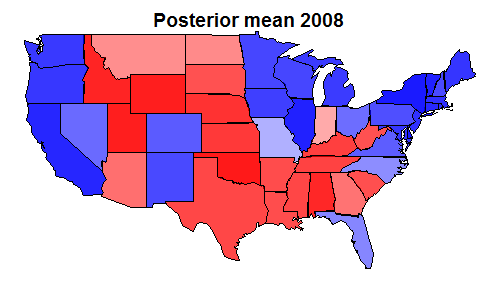
\includegraphics[scale=.70]{08pred.png}\\
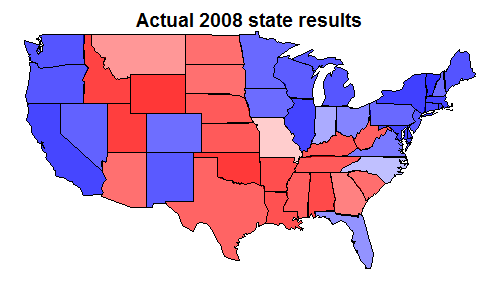
\includegraphics[scale=.70]{08actual.png}\\

\indent Analysis of the predicted versus actual state maps reveals a couple of interesting observations about the model. Our predictions were nearly all accurate at the state level except for Missouri and Indiana, which were predicted to be Republican and Democratic, respectively. The net result of these two incorrect predictions is to give the Republican candidate one extra vote, because Indiana has 1 more electoral vote than Missouri.

\indent We can also see that our model tends to overestimate the margin of victory for both candidates; our marginal posterior mean plot tends to be the same color but darker than the corresponding actual results. In general, we tend to correctly predict the state-level winners but overestimate the winner's margin of victory.

\indent A histogram of the sample taken from our converged posterior distribution for the 2008 election is shown below:\\
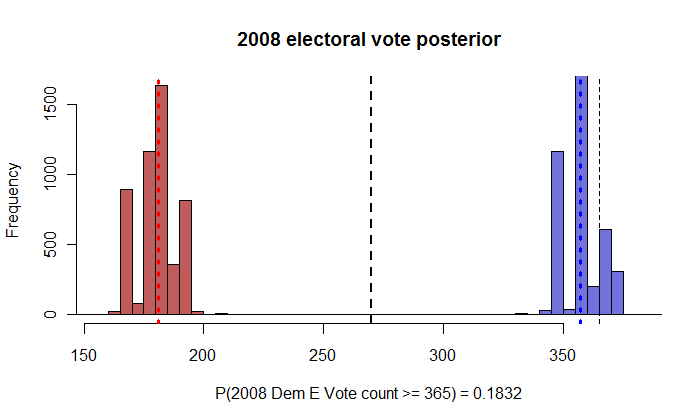
\includegraphics[scale=.50]{08hist.png}\\

%[Include Actual and Predicted Political Maps Here]

\subsection{Sensitivity Analysis}
\hspace{31pt} We also tested the prediction accuracy of our model using an uninformative prior ($b_{ij}$ = 50/3), in which case we concluded that Barrack Obama would win the 2008 election with a central 95\% interval of [347, 371] electoral votes and a median of 357 votes. These results are identical to our results obtained when utilizing and informative prior.

%2012 RESULTS
\pagebreak
\section{Results \& Conclusion}

\subsection{General Results}
\hspace{31pt} In an analysis of the 2012 election, we predicted that Barrack Obama will win the election with 99.9\% probability, inside the central 95\% interval of [285,332] electoral votes, with a median of 303 electoral votes, and with a mean of 307.8 electoral votes.

\indent The general 2012 results are shown graphically below:\\
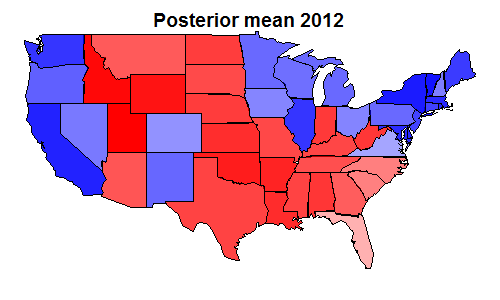
\includegraphics[scale=.70]{12pred.png}\\
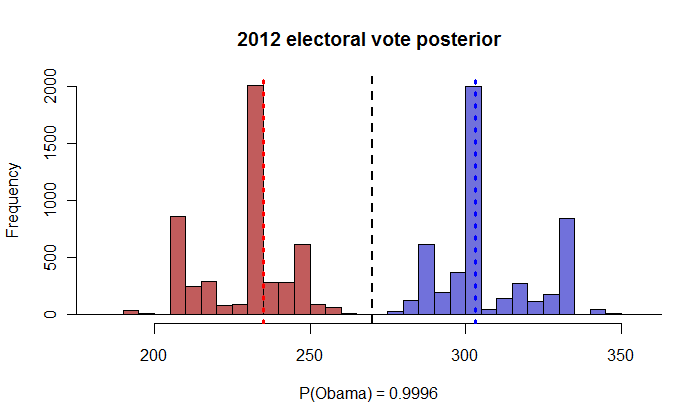
\includegraphics[scale=.50]{12hist.png}\\


%Romney Optimistic
\subsection{Romney-Optimistic Scenario}
\hspace{31pt} We also attempted to model a Romney-Optimistic scenario by maximizing Mitt Romney's probability of winning the election with respect to the tuning parameters of limiting the poll range (as discussed in {\bf 3.6 Parameter Tuning}). Hence, by using only the 3 most recent polls, we found that Barrack Obama will win the election with 96.7\% probability and a 95\% central interval of [269,332] electoral votes. 

\indent The Romney-Optimistic results are shown graphically below:\\
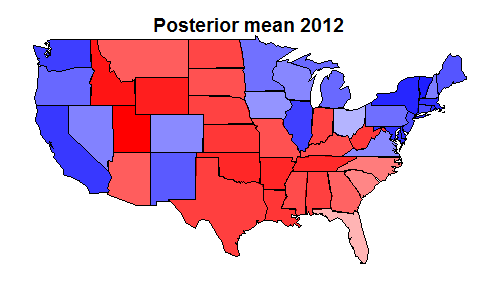
\includegraphics[scale=.70]{12predrom.png}\\
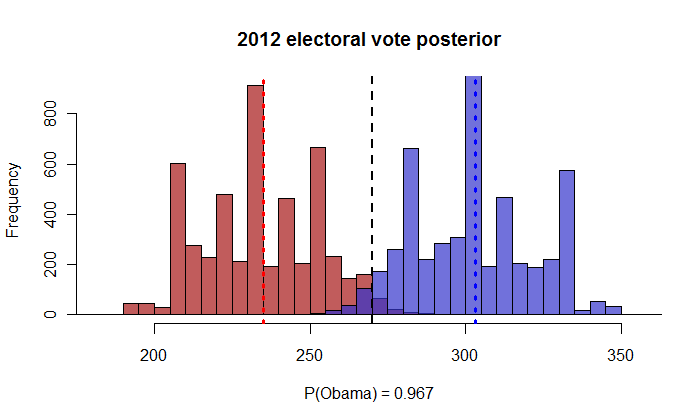
\includegraphics[scale=.50]{12histrom.png}\\

\pagebreak
\indent In particular, we found that Ohio is the only swing state whose mean differentials in the 3.3\% of Romeny-Optimistic posterior samples in which Mitt Romney wins the election and whose mean differentials in the 96.7\% of samples in which Barrack Obama wins had opposite signs (where the mean differential for state $j$ is defined as $\hat p_{1j} - \hat p_{2j}$). Hence, if, a priori, we gave Ohio to Mitt Romney, we found that his chances of winning the election were increased to roughly 22\%, as shown below:\\

\noindent 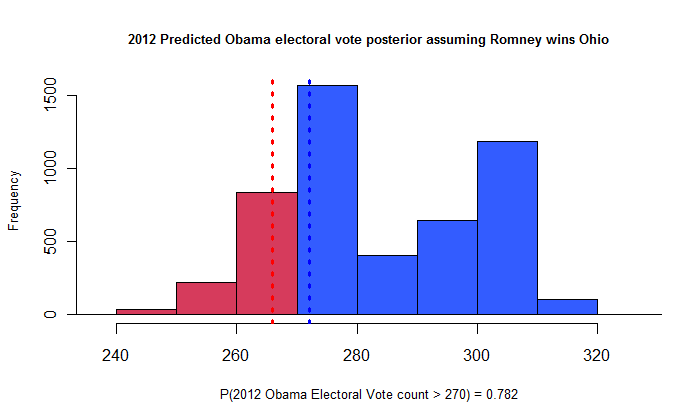
\includegraphics[scale=.50]{12ohio.png}\\

%Sensitivity Analysis
\subsection{Sensitivity Analysis}
\hspace{31pt} We also tested the prediction accuracy of our general and Romney-Optimistic models using  uninformative priors. For the general model, we concluded that Barrack Obama will win the 2012 election with a central 95\% interval of [285, 332] electoral votes, a median of 303 electoral votes, and a mean of 307.8 electoral votes.\\
\indent Our results for the Romney-Optimistic scenario utilizing an uninformative prior gave Barrack Obama a central 95\% interval of [270, 332] electoral votes, a median of 303 electoral votes, a  mean of 303.3 electoral votes, and an overall 97.24\% chance of winning.\\
\indent Both of these results are nearly identical to the results obtained from the models utilizing informative priors.

%REFERENCES
\pagebreak
\section{References}
\parindent 15pt
Jackman, S., \& Rivers, D. (2001). \emph{State-level election forecasting during}\\
\indent \emph{election 2000 via dynamic Bayesian hierarchical modeling} (Working Paper).\\
\indent Stanford, CA: Stanford University, Department of Political Science.\\
Kaplan, E., \& Barnett, A. (2003). A new approach to estimating the probability\\
\indent of winning the presidency. \emph{Operations Research}, 51(1), 32-40.\\
Rigdon, Steven E. (2009). A Bayesian Prediction Model for the U.S.\\
\indent Presidential Election. \emph{American Politics Research}, 37(4), 700-724.

%CONVERGENCE PLOTS
\section{Appendix (Convergence Examples)}
\subsection{California, Colorado, and Connecticut}
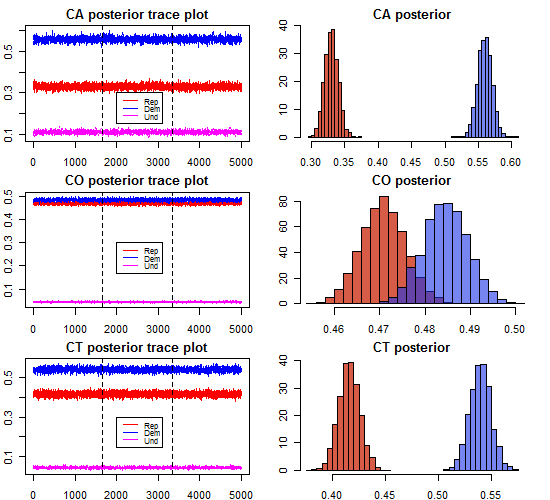
\includegraphics[scale=.60]{trace1.png}\\

\pagebreak
\subsection{Florida, Georgia, and Hawaii}
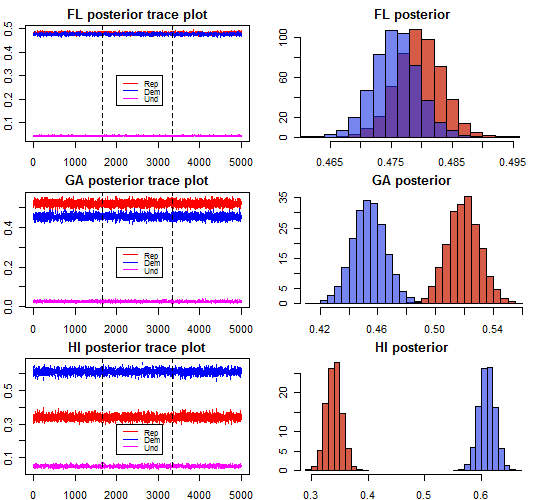
\includegraphics[scale=.60]{trace2.png}\\

\pagebreak
\subsection{Vermont, Virginia, and Washington}
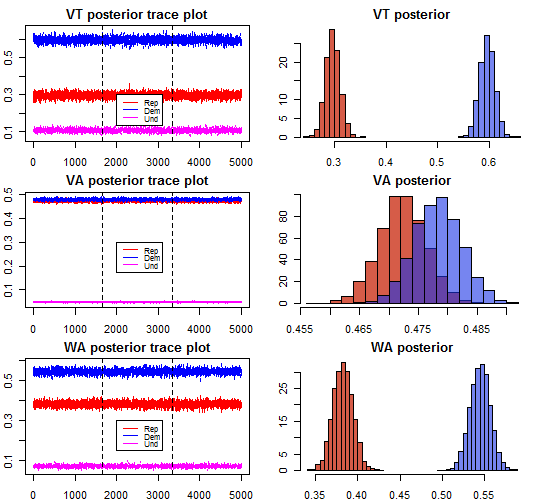
\includegraphics[scale=.60]{trace3.png}

\end{document}